% !TEX root = ../discretemath.tex

\section{Стандартные таблицы Юнга и формула крюков}

Число стандартных таблиц Юнга формы $\lambda$ даётся формулой крючков Фрейма–Робинсона–Тролла: $f_\lambda=n!/\prod_\square h(\square)$. Ниже — определения, формула и скетч доказательства (индукция по $n$ с тождеством через интерполяцию Лагранжа).

\subsection{Стандартные таблицы Юнга}

\begin{Definition}{Стандартная таблица Юнга (СТЮ)}{}
	\emph{СТЮ} формы $\lambda$ ($|\lambda|=n$) — расстановка чисел $1,\dots,n$ по клеткам $\lambda$ (по одному), строго возрастающая вдоль каждой строки (слева направо) и каждого столбца (сверху вниз). $f_\lambda=\#\{\text{СТЮ формы }\lambda\}$.
\end{Definition}

\begin{Example}{}{}
	Для $\lambda=(2,2,1)$ ($n=5$) ровно $5$ таблиц:
	\begin{center}
		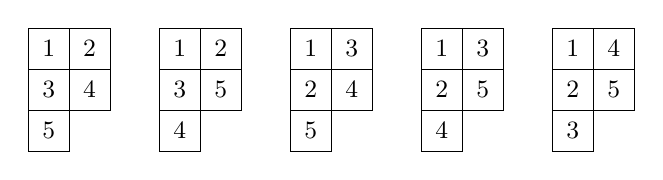
\begin{tikzpicture}[scale=0.52]
			\foreach \xoff/\avals in {%
				0/{0/0/1,0/1/2,1/0/3,1/1/4,2/0/5},%
				3.2/{0/0/1,0/1/2,1/0/3,1/1/5,2/0/4},%
				6.4/{0/0/1,0/1/3,1/0/2,1/1/4,2/0/5},%
				9.6/{0/0/1,0/1/3,1/0/2,1/1/5,2/0/4},%
				12.8/{0/0/1,0/1/4,1/0/2,1/1/5,2/0/3}}{
				\begin{scope}[xshift=\xoff cm]
					\foreach \r/\c/\v in \avals {
						\draw (\c,-\r) rectangle (\c+1,-\r+1);
						\node[font=\small] at (\c+0.5,-\r+0.5) {\v};
					}
				\end{scope}
			}
		\end{tikzpicture}
	\end{center}
\end{Example}

\subsection{Формула крючков}

\begin{Definition}{Крюк клетки}{}
	\emph{Крюк} клетки $\square=(i,j)\in\lambda$:
	\[
	\mathrm{Hook}(\square)=\{(i,j)\}\cup\{(i,j'):j'>j\}\cup\{(i',j):i'>i\}\quad(\text{в пределах }\lambda),
	\]
	то есть сама клетка, «рука» (правее в строке) и «нога» (ниже в столбце). Длина крюка $h(\square)=|\mathrm{Hook}(\square)|$.
\end{Definition}

\begin{center}
	\begin{tikzpicture}[scale=0.48]
		\foreach \col in {1,...,5} { \draw (\col-1,3) rectangle (\col,4); }
		\foreach \col in {1,...,4} { \draw (\col-1,2) rectangle (\col,3); }
		\foreach \col in {1,...,3} { \draw (\col-1,1) rectangle (\col,2); }
		\draw (0,0) rectangle (1,1);
		\fill[blue!22] (0,2) rectangle (4,3);
		\fill[blue!22] (0,0) rectangle (1,2);
		\draw[very thick,blue] (0,2) rectangle (1,3);
		\node[blue,font=\small] at (0.5,2.5) {$\square$};
		\node[right,font=\small] at (5.4,2.5) {крюк клетки $\square$, $h(\square)=6$};
	\end{tikzpicture}
\end{center}

\begin{Theorem}{Формула крючков (Frame–Robinson–Thrall, 1954)}{}
	Число СТЮ формы $\lambda$ ($|\lambda|=n$):
	\[
	f_\lambda=\frac{n!}{\prod_{\square\in\lambda}h(\square)}.
	\]
\end{Theorem}

\begin{Example}{}{}
	Для $\lambda=(2,2,1)$ длины крюков:
	\begin{center}
		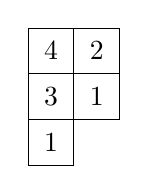
\begin{tikzpicture}[scale=0.58]
			\foreach \r/\c/\v in {0/0/4,0/1/2,1/0/3,1/1/1,2/0/1}{
				\draw (\c,-\r) rectangle (\c+1,-\r+1);
				\node at (\c+0.5,-\r+0.5) {\v};
			}
		\end{tikzpicture}
	\end{center}
	\[
	f_{(2,2,1)}=\frac{5!}{4\cdot 3\cdot 2\cdot 1\cdot 1}=\frac{120}{24}=5.
	\]
\end{Example}

\subsection{Скетч доказательства}

\begin{Lemma}{Рекуррента по углам}{}
	\[
	f_\lambda=\sum_{\mu=\lambda\setminus\square}f_\mu,
	\]
	сумма по диаграммам $\mu$, полученным удалением одной \textbf{угловой} клетки $(i,j)$ (с $(i,j+1)\notin\lambda$ и $(i+1,j)\notin\lambda$).
\end{Lemma}

\begin{proof}
	В СТЮ число $n$ стоит в угловой клетке (иначе нарушится монотонность). Удаление этой клетки даёт СТЮ формы $\mu$ с числами $\{1,\dots,n-1\}$; это биекция.
\end{proof}

Индукция по $n$. \textbf{База} $n=1$: $f_\square=1=1!/1$. \textbf{Переход:} по лемме и ИП достаточно показать
\begin{equation}\tag{$*$}
	\sum_{i=1}^{k}\frac{\prod_{\square\in\lambda}h(\square)}{\prod_{\square\in\lambda\setminus\alpha_i}h_{\lambda\setminus\alpha_i}(\square)}=n,
\end{equation}
где $\alpha_1,\dots,\alpha_k$ — все угловые клетки.

\begin{Definition}{Содержание клетки}{}
	$c(i,j)=j-i$.
\end{Definition}

\begin{center}
	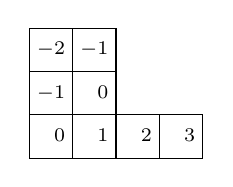
\begin{tikzpicture}[scale=0.55]
		\foreach \r/\c/\v in {%
			0/0/{$-2$}, 0/1/{$-1$},%
			1/0/{$-1$}, 1/1/{$\phantom{-}0$},%
			2/0/{$\phantom{-}0$}, 2/1/{$\phantom{-}1$}, 2/2/{$\phantom{-}2$}, 2/3/{$\phantom{-}3$}%
		}{
			\draw (\c,-\r) rectangle (\c+1,-\r+1);
			\node[font=\scriptsize] at (\c+0.5,-\r+0.5) {\v};
		}
	\end{tikzpicture}
\end{center}

Пусть $x_i=c(\alpha_i)$ (углы), $x_1<\dots<x_k$, а между ними — \emph{добавляемые} клетки $\beta_0,\dots,\beta_k$ с содержаниями $y_j=c(\beta_j)$, перемежающимися: $y_0<x_1<y_1<\dots<x_k<y_k$.

\begin{center}
	\begin{tikzpicture}[scale=0.46]
		\draw[thick] (0,0) rectangle (7,1);
		\draw[thick] (0,1) rectangle (6,2);
		\draw[thick] (0,2) rectangle (5,3);
		\draw[thick] (0,3) rectangle (3,4);
		\draw[thick] (0,4) rectangle (2,5);
		\draw[thick] (0,5) rectangle (1,6);
		\foreach \x in {1,...,6} \draw[thick] (\x,0)--(\x,1);
		\foreach \x in {1,...,5} \draw[thick] (\x,1)--(\x,2);
		\foreach \x in {1,...,4} \draw[thick] (\x,2)--(\x,3);
		\foreach \x in {1,...,2} \draw[thick] (\x,3)--(\x,4);
		\draw[thick] (1,4)--(1,5);
		\fill[red!35] (0,5) rectangle (1,6);  \node[font=\tiny] at (0.5,5.5) {$\beta_0$};
		\fill[blue!35] (1,4) rectangle (2,5); \node[font=\tiny] at (1.5,4.5) {$\alpha_1$};
		\fill[red!35] (2,3) rectangle (3,4);  \node[font=\tiny] at (2.5,3.5) {$\beta_1$};
		\fill[blue!35] (3,2) rectangle (4,3); \node[font=\tiny] at (3.5,2.5) {$\alpha_2$};
		\fill[red!35] (5,1) rectangle (6,2);  \node[font=\tiny] at (5.5,1.5) {$\beta_2$};
		\fill[blue!35] (6,0) rectangle (7,1); \node[font=\tiny] at (6.5,0.5) {$\alpha_k$};
		\draw[dashed,thick] (7,0) rectangle (8,1); \node[font=\tiny] at (7.5,0.5) {$\beta_k$};
		\node[right,font=\small] at (8.5,3) {$\alpha_1,\dots,\alpha_k$ — углы};
		\node[right,font=\small] at (8.5,2) {$\beta_0,\dots,\beta_k$ — добавляемые};
	\end{tikzpicture}
\end{center}

\textbf{Ключевое свойство:} $\sum_{i=1}^k x_i=\sum_{j=0}^k y_j$ (то есть $e_1(\bar x)=e_1(\bar y)$).

\paragraph{Отношение произведений крюков.}
Анализ изменения длин крюков при удалении $\alpha_i$ даёт
\[
\frac{\prod_{\square\in\lambda}h(\square)}{\prod_{\square\in\lambda\setminus\alpha_i}h_{\lambda\setminus\alpha_i}(\square)}
=\frac{\prod_{j=0}^{k}(x_i-y_j)}{\prod_{j\neq i}(x_i-x_j)}.
\]

\paragraph{Ключевое тождество.}
Положим $g(\bar x,\bar y)=\sum_{i=1}^{k}\dfrac{\prod_{j=0}^{k}(x_i-y_j)}{\prod_{j\neq i}(x_i-x_j)}$.

\begin{Statement}{}{}
	$g(\bar x,\bar y)=-n$.
\end{Statement}

\begin{proof}[Скетч]
	\textbf{1.} $g$ — многочлен (особенности при $x_i\to x_j$ сокращаются телескопически). \textbf{2.} Степень каждого слагаемого $(k+1)-(k-1)=2$, поэтому $\deg g\le 2$. \textbf{3.} Интерполяция Лагранжа: для $P(x)=\prod_{j=0}^k(x-y_j)=x^{k+1}-e_1(\bar y)x^k+e_2(\bar y)x^{k-1}-\cdots$
	\[
	\sum_{i=1}^k\frac{P(x_i)}{\prod_{j\neq i}(x_i-x_j)}=h_2(\bar x)-e_1(\bar y)h_1(\bar x)+e_2(\bar y),
	\]
	где $h_m$ — полные симметрические функции. Используя $e_1(\bar x)=e_1(\bar y)$, получаем $g=e_2(\bar x)-e_2(\bar y)$. \textbf{4.} Из $e_1(\bar x)=e_1(\bar y)$ следует $\sum x_i^2+2e_2(\bar x)=\sum y_j^2+2e_2(\bar y)$, откуда $g=\dfrac{\sum y_j^2-\sum x_i^2}{-2}$. Для диаграмм Юнга справедливо $\sum_j c(\beta_j)^2-\sum_i c(\alpha_i)^2=2n$ (индукция по добавлению клетки). Значит, $g=-2n/2=-n$.
\end{proof}

Следовательно, левая часть $(*)$ равна $-g=n$, и по индукции формула крючков доказана.
